\section{Background of the Study}

Mangoes, also known as the Mangifera indica, are a member of the cashew family. 
This fruit can often be seen being farmed by countries such as Myanmar, the Philippines, 
and India as they have a tropical dry season. Being in a tropical country is an important 
aspect for mango cultivation as it ensures proper growth for mangoes. 
If aspects such as temperature and rainfall are not ideal, it may affect the quality 
of the mango \citep{noauthor-mango-2024}. 
\begin{figure}[!htbp]
	\centering
		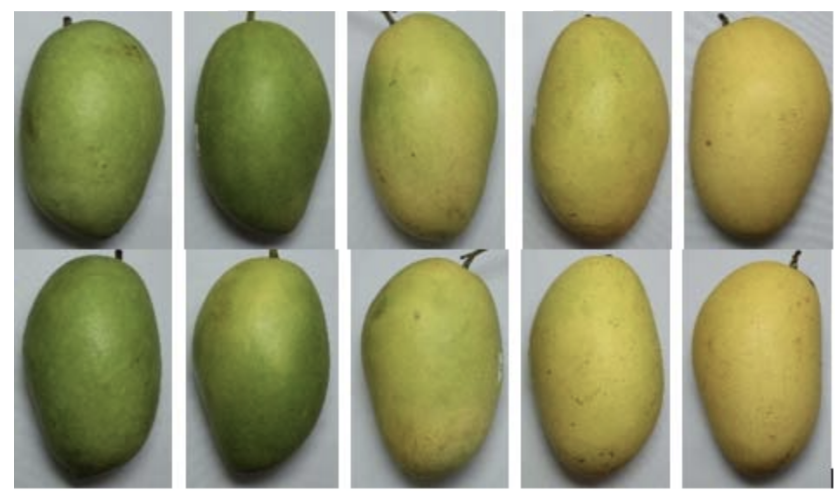
\includegraphics[width=0.5\textwidth]{fig1}
	\caption{Carabao Mangoes at Different Ripeness Stages \citep{guillermo-determining-2019}}
	\label{fig:img1}
\end{figure}
Carabao mangoes is a variety of a mango that is found and cultivated in the Philippines. It is known for its sweet signature taste that was recognized sweetest in the world in the Guinness Book of World Records in 1995. The mango was named after the national animal of the Philippines, a native breed of buffalo. On average, it is 12.5 cm in length and 8.5 cm in diameter, having a bright yellow color when ripe as seen in Figure 1.1. It is often cultivated during late May to early July \citep{DBpediaCarabao}.

As the Philippines is a tropical country, mangoes are a highly valued fruit as it is not only the country’s national fruit but also amongst the leading agricultural exports of the country, ranking only third below bananas and pineapples. This gives the country the 9th slot amongst the leading exporters of Mangoes across the world. Attributed to this ranking is the country's export of both fresh and dried mangoes, as well as low tariff rates. This allows the country to export a large quantity of the fruit in countries such as Singapore, Japan, and the USA as they can enter duty free markets provided by the World Trade Organization and Japan. Due to this, the mangoes have become a major source of income to an estimated 2.5 million farmers in the country \citep{centino-current-nodate}.

Before mangoes are sold in markets, they first undergo multiple post-harvest processes. This is to ensure that the mangoes that arrive in markets are utmost quality before being sold to consumers. Moreover, it ensures that mangoes are contained and preserved properly such that they do not incur damages and/or get spoiled on its transportation to the market. Processing of the mango involves pre-cooling, cleaning, waxing, classification, grading, ripening, packaging, preservation, storage, packing, and transportation \citep{patel-novel-2019} \citep{rizwan-iqbal-classification-2022}.

Among the processes that mangoes undergo, classification and grading is important as it allows the manufacturer to separate mangoes with good qualities versus mangoes with poor qualities. According to a study by \citep{lacap-bruise-2021}, size, length, width, volume, density, indention, and grooves are aspects that determine the maturity of mangoes. These traits are being checked along with the ripeness of the mango, sightings of bruise injury, and cracks on the fruit \citep{lacap-bruise-2021} as these aspects affect the sellability of the fruit as well as the chances of it getting spoiled sooner.

Previous studies have been made to automate the sortation process of the mangoes. Among these is a research done by \citet{abbas-mango-2018}, which focuses on classification of mangoes using their texture and shape features. They do this by, first, acquiring an image of the mango using a digital camera. Then, these images are fed to the MaZda package, which is a software originally developed for magnetic resonance imaging. Within the MaZda package is the B11 program, which uses Principal Component Analysis, Linear Discriminant Analysis, Nonlinear Discriminant Analysis, and texture classification to extract features from the mango, which in this case are the length, width, and texture. This data is then compared to a database in order to classify any given mango \citep{abbas-mango-2018}.  

Another study is done by \citet{rizwan-iqbal-classification-2022}, which classifies mangoes based on their color, volume, size, and shape This is done by making use of Charge Coupled Devices, Complementary Metal-Oxide Semiconductor sensors, and 3-layer Convolutional Neural Network. To classify the mangoes, images are first captured and preprocessed to be used as a data set \citep{rizwan-iqbal-classification-2022}. This data set is then augmented to be used as a model for the 3-layer Convolutional Neural Network. After extracting the features of the mango, the 3-layer Convolutional Neural Network is used as a method for their classification as it can mimic the human brain in pattern recognition, and process data for decision making. This is important as some mangoes have very subtle differences which make it difficult to differentiate them.



\section{Prior Studies}

A paper written by \citet{amna-et-al-machine-2023}, designed an automated fruit sorting machine based on the quality through 
an image acquisition system and CNN. Furthermore, the results of the paper show that the image processing detection 
score was 89\% while that of the tomatoes was 92\% while the CNN model had higher validity of 95\% for mangoes and 93\% 
for tomatoes. 15\%, while the percentage of distinction between the two groups was reported to be 5\% respectively 
\citep{amna-et-al-machine-2023}. Despite the high \gls{accuracy score}  in detecting mango defects, the fruit sorting system only sorts based 
on the mango defects and not on ripeness, and weight.

Furthermore, the research paper presented by \citet{guillergan-naive-2024} designed an Automated Carabao mango classifier, 
in which the mango image database is used to extract the features like size, area along with the ratio of the spots for 
grading using Naïve Bayes Model. For the results, the Naïve Bayes’ model recognized large and rejected mangoes with 95\%
 accuracy and the large and small/medium difference with a 7\% error, suggesting an application for quality differentiation 
 and sorting in the mango business industry. Despite the high accuracy of classifying Carabao mangoes, the researchers used a 
 high quality DSLR camera for the image acquisition system without any \gls{microcontroller} to control the mangoes \citep{guillergan-naive-2024}. 


\section{Problem Statement}
As mangoes are among the top exports of the Philippines \citep{centino-current-nodate}, 
assessing the physical deformities is a necessity. The physical deformities of the 
Carabao mango can determine the global competitiveness of the country. Having higher quality
 exports can often lead to gaining competitive edge, increase in demand, increase export revenues,
  and becoming less susceptible to low-wage competition \citep{dadamo-determinants-2018}. In order to increase the 
  quality of mango fruit exports, a key post-harvest process is done, which is sorting and grading.
   Mango sorting and grading then becomes important to determine which batches are of high quality and
    can be sold for a higher price, and which batches are of low quality and can only be sold for a low price
	 \citep{zhengzhou-first-industry-co-ltd-what-nodate}. Traditionally, fruit sorting and grading is inefficient as it is
	  done manually by hand. Some tools are used such as porous ruler to determine fruit size and color palette 
	  for color grading \citep{zhengzhou-first-industry-co-ltd-what-nodate}. However, among the problems encountered in the 
	  process of manually sorting and grading mangoes are susceptibility to human error and requiring a number of 
	  laborers to do the task. 

	  With the current advancements in technology, some researchers have already taken steps to automate the process
	   of sorting and grading mangoes. However, these attempts would often only consider some of the aspects 
	   pertaining to size, ripeness, and \gls{bruises} but not all of them at the same time. Lastly, not all research approaches
	    were able to implement a hardware for their algorithm, limiting their output to only a software implementation and not
		 an embedded system. As such the proposed system would assess the export quality of the Carabao mango based on all the
		  mentioned mango traits, namely size, \gls{bruises}, and ripeness while also taking into consideration being non-destructive.
		   These aspects are important because, as was previously mentioned, there is a need to develop a Carabao mango sorter 
		   that takes into account all these aspects at the same time while being non-destructive.



\section{Objectives and Deliverables}

\subsection{General Objective (GO)}
\begin{itemize}
	\item \Copy{GO}{GO: To develop a user-priority-based grading and sorting system for Carabao mangoes, 
 using machine learning and computer vision techniques to assess ripeness, size, and bruises. };
\end{itemize}

\subsection{Specific Objectives (SOs)}

\begin{itemize}
	\item \Copy{SO1}{SO1: To make an image acquisition system with a conveyor belt for 
	automatic sorting and grading mangoes. };
	
	\item \Copy{SO2}{SO2: To get the precision, recall, F1 score, confusion matrix,
	 and train and test accuracy metrics for classifying the ripeness and bruises with an accuracy score of at least 90\%.};
	
	\item \Copy{SO3}{SO3: To create a microcontroller-based system to operate the image acquisition system, 
	control the conveyor belt, and process the mango images through machine learning. };

	\item \Copy{SO4}{SO4: To grade mangoes based on user priorities for size, ripeness, and bruises.  };
	
	\item \Copy{SO5}{SO5: To classify mango ripeness based on image data using machine learning algorithms
	 such as kNN, k-mean, and Naïve Bayes.  };
	
	\item \Copy{SO6}{SO6: To classify mango size based on image data by getting its length and width using OpenCV, 
	geometry, and image processing techniques. };

	\item \Copy{SO7}{SO7: To classify mango bruises based on image data by employing machine learning algorithms.}
\end{itemize}

%\Copy{SO9}{To classify mango bruises based on image data by employing machine learning algorithms.}


\subsection{Expected Deliverables}

Table~\ref{tab:expd1} and ~\ref{tab:expd2} shows the outputs, 
products, results, achievements, gains, realizations, and/or
yields of the \documentType. 

\begin{table}[!htbp]
	\caption{Expected Deliverables per Objective} 	
	\label{tab:expd1} 
	{\centering \scriptsize
		\begin{tabular}{p{0.3\textwidth}|p{0.6\textwidth}}
			\hline 
			\hline 
			\textbf{Objectives} & 
			\textbf{Expected Deliverables}\\ 
			\hline 
%%			\endfirsthead
%			\multicolumn{2}{c}%
%			{\textit{Continued from previous page}} \\
%			\hline
%			\hline 
%			\textbf{Objectives} & 
%			\textbf{Expected Deliverables}\\ 
%			\hline 
%%			\endhead
%			\hline 
%			\multicolumn{2}{r}{\textit{Continued on next page}} \\ 
%%			\endfoot
%			\hline 
%%			\endlastfoot
%			\hline		
			\Paste{GO} &
			\begin{minipage}{0.55\textwidth}
				\vspace{10pt} 
				\begin{itemize}
					\item To develop a Carabao mango grading and sorting system 
					\item To grade Carabao mangoes into three categories based on ripeness, size, and 
					bruises of the Carabao mangoes using machine learning.
					\item To integrate sensors and actuators to control the conveyor belt and image acquisition system.
				\end{itemize}
			\end{minipage} \\ \hline

			\Paste{SO1} & 
			\begin{minipage}{0.55\textwidth}
				\vspace{10pt}
				\begin{itemize}
					\item To make an image acquisition system with a camera and LED light source.
					\item To build a flat belt conveyor for moving the mangoes.
				\end{itemize}
			\end{minipage} \\ \hline

			\Paste{SO2} & 
			\begin{minipage}{0.55\textwidth}
				\vspace{10pt}
				\begin{itemize}
					\item To use a publicly available dataset of at least 10,000 mango images
					 for classification of ripeness, and bruises.
				\end{itemize}
			\end{minipage} \\ \hline
						
			\Paste{SO3} & 
			\begin{minipage}{0.55\textwidth}
				\vspace{10pt}
				\begin{itemize}
					\item To develop an intuitive UI where users can start and stop the system.
					\item To implement a priority-based grading system with sliders for ripeness, bruises, and size.
				\end{itemize}
			\end{minipage} \\ \hline
						
			\Paste{SO4} & 
			\begin{minipage}{0.55\textwidth}
				\vspace{10pt}
				\begin{itemize}
					\item To utilize a linear combination formula as the overall mango score, where each classification level 
					contributes a grade, weighted by the priority assigned to the three properties.
					\item To assign score values for each classification level of the mango.
				\end{itemize}
			\end{minipage} \\ \hline
		

			\Paste{SO5} & 
			\begin{minipage}{0.55\textwidth}
				\vspace{10pt}
				\begin{itemize}
					\item To train a machine learning model such as kNN, k-mean, naive Bayes capable
					of classifying mango ripeness based on the image color
					\item To gather a dataset of annotated images with ripeness labels
					\item To obtain an evaluation report of performance metrics of the model
				\end{itemize}
			\end{minipage} \\ \hline

			
		\end{tabular}	
			
	}
\end{table}


\begin{table}[!htbp]
	\caption{Expected Deliverables per Objective continued} 	
	\label{tab:expd2} 
	{\centering \scriptsize
		\begin{tabular}{p{0.3\textwidth}|p{0.6\textwidth}}
			\hline 
			\hline 
			\textbf{Objectives} & 
			\textbf{Expected Deliverables}\\ 
			\hline 
			\Paste{SO6} & 
			\begin{minipage}{0.55\textwidth}
				\vspace{10pt}
				\begin{itemize}
					\item To develop an image processing algorithm capable of determining mango 
					size using OpenCV, NumPy, and imutils
					\item To classify mangoes based on size and categories into small, medium, 
					and large based on those measures
				\end{itemize}
			\end{minipage} \\ \hline

			\Paste{SO7} & 
			\begin{minipage}{0.55\textwidth}
				\vspace{10pt}
				\begin{itemize}
					\item To train a machine learning model such as 
					CNN capable of distinguishing bruised and non-bruised mangoes
					\item To train a machine learning model such as kNN, k-mean, and Naïve Bayes 
					capable of assessing the extent of bruising on the mangoes if it is significant or partial
					\item To gather a dataset of annotated images based on bruises
					\item To obtain an evaluation report of performance metrics of both CNN and machine learning models
				\end{itemize}
			\end{minipage} \\ \hline
		\end{tabular}
	}
\end{table}


% \begin{center}
% 	{\scriptsize
% 		\begin{longtable}{p{0.2\textwidth}|p{0.6\textwidth}|p{0.1\textwidth}}
% 			\caption{Summary of methods for reaching the objectives} \label{tab:methods_per_objective} \\
% 			\hline 
% 			\hline 
% 			\textbf{Objectives} & 
% 			\textbf{Expected Deliverables} &
% 			\textbf{Locations}\\ 
% 			\hline 
% 			\endhead
% 			\hline 
% 			\multicolumn{3}{r}{\textit{Continued on next page}} \\ 
% 			\endfoot
% 			\hline 
% 			\endlastfoot
% 			\hline
% 			\Paste{GO} & \begin{itemize}
% 				\item To develop a Carabao mango grading and sorting system 
% 				\item To grade Carabao mangoes into three categories based on ripeness, size, and 
% 				bruises of the Carabao mangoes using machine learning.
% 				\item To integrate sensors and actuators to control the conveyor belt and image acquisition system.
% 			\end{itemize} & Sec.~\ref{sec:implement} on p.~\pageref{sec:implement}\\ \hline
			
% 			\Paste{SO1} & \begin{itemize}
% 				\item To make an image acquisition system with a camera and LED light source.
% 				\item To build a flat belt conveyor for moving the mangoes.
% 			\end{itemize} & Sec.~\ref{sec:implement} on p.~\pageref{sec:implement} \\ \hline
			
% 			\Paste{SO2} & \begin{itemize}
% 				\item To use a publicly available dataset of at least 10,000 mango images
% 				 for classification of ripeness, and bruises.
% 			\end{itemize} & Sec.~\ref{sec:implement} on p.~\pageref{sec:implement}\\ \hline
			
% 			\Paste{SO3} & \begin{itemize}
% 				\item To develop an intuitive UI where users can start and stop the system.
% 				\item To implement a priority-based grading system with sliders for ripeness, bruises, and size.
% 			\end{itemize} & Sec.~\ref{sec:implement} on p.~\pageref{sec:implement}\\ \hline
			
% 			\Paste{SO4} & \begin{itemize}
% 				\item To utilize a linear combination formula as the overall mango score, where each classification level 
% 				contributes a grade, weighted by the priority assigned to the three properties.
% 				\item To assign score values for each classification level of the mango.
% 			\end{itemize} & Sec.~\ref{sec:implement} on p.~\pageref{sec:implement} \\ \hline
			
% 			\Paste{SO5} & \begin{itemize}
% 				\item To train a machine learning model such as kNN, k-mean, naive Bayes capable
% 				of classifying mango ripeness based on the image color
% 				\item To gather a dataset of annotated images with ripeness labels
% 				\item To obtain an evaluation report of performance metrics of the model
% 			\end{itemize} & Sec.~\ref{sec:implement} on p.~\pageref{sec:implement} \\ \hline

% 			\Paste{SO6} & \begin{itemize}
% 				\item To develop an image processing algorithm capable of determining mango 
% 				size using OpenCV, NumPy, and imutils
% 				\item To classify mangoes based on size and categories into small, medium, 
% 				and large based on those measures
% 			\end{itemize} & Sec.~\ref{sec:implement} on p.~\pageref{sec:implement} \\ \hline

% 			\Paste{SO7} & \begin{itemize}
% 				\item To train a machine learning model such as 
% 				CNN capable of distinguishing bruised and non-bruised mangoes
% 				\item To train a machine learning model such as kNN, k-mean, and Naïve Bayes 
% 				capable of assessing the extent of bruising on the mangoes if it is significant or partial
% 				\item To gather a dataset of annotated images based on bruises
% 				\item To obtain an evaluation report of performance metrics of both CNN and machine learning models
% 			\end{itemize} & Sec.~\ref{sec:implement} on p.~\pageref{sec:implement} \\ \hline
			
% 		\end{longtable}
% 	}
% \end{center}

\section{Significance of the Study}

Automating the process of sorting and grading mangoes increases efficiency and 
productivity for the user which would in effect remove human error in sorting and
 grading and decrease the human labor and time taken to sort and grade the mangoes.
  This is especially important for farmers with a large amount of fruit such as mangoes and a
   lesser labor force. A recent study showed that
    their automated citrus sorter and grader using computer vision can reduce the human
	 labor cost and time to sort and grade when comparing the automated citrus sorter and grader
	  to manual human labor \cite{chakraborty-development-2023}. 

Another benefit to automating sorting and grading mangoes is the improvement in quality control.
 This implies that compared to human labor, automating sorting and grading mangoes can uniformly 
 assess the quality of mangoes based on size, color, and \gls{bruises}, ensuring that the expected grade and high-quality mangoes reach the consumer. By accurately identifying substandard mangoes, the system 
  helps in reducing waste and ensuring that only marketable fruits are processed further.

Likewise, the scalability of automating sorting and grading mangoes is simpler, especially 
for lower labor force farmers with large volumes of mangoes. Because of the possibility of
 large-scale operations by automating sorting and grading mangoes, farmers can now handle large
  volumes of mangoes, making them suitable for commercial farms and processing plants. Moreover,
   it can be adapted to different varieties of mangoes and potentially other fruits with minor modifications.


\subsection{Technical Benefit}

\begin{enumerate}
	\item The development of an automated \gls{Carabao mango} sorter would increase the quality control 
	of classifying \gls{Carabao mango} based on ripeness, size, and bruising.
	
	\item The accuracy in sorting Carabao mangoes will be significantly improved while
	 reducing the errors due to human factors in manual sorting.
	
	\item The automated \gls{Carabao mango}  sorter carefully sorts the mangoes 
	while ensuring that they remain free from bruising or further damage during the process	
\end{enumerate}

\subsection{Social Impact}

\begin{enumerate}
	\item The reduction in manual labor creates opportunities in maintenance and
	 technologies in the automated \gls{Carabao mango}  sorter.
	
	\item The automated \gls{Carabao mango}  sorter system improves Carabao mango 
	standards and enhances the satisfaction of the buyers and the customers through
	 guaranteeing consistent Carabao mango grade.
	
	\item Opportunity to increase sales and profit for the farmers through consistent 
	quality and grade Carabao mangoes while reducing the physical labor to sort it.
\end{enumerate}

\subsection{Environmental Welfare}

\begin{enumerate}
	\item With the utilization of non-destruction methods of classifying Carabao mangoes together with an
	 accurate sorting system, overall waste from Carabao mangoes is reduced and the likelihood
	  of improperly sorted mangoes is decreased.
	
	\item Automation of sorting and grading Carabao mangoes promotes sustainable farming practices.
	
\end{enumerate}



\section{Assumptions, Scope, and Delimitations}

\subsection{Assumptions}

\begin{enumerate}
	\item The Carabao mangoes are from the same source together with the same variation
	
	\item The Carabao mangoes do not have any fruit borer and diseases
	
	\item All the components do not have any form of defects
	\item The prototype would have access to constant electricity/power source.
	\item The Carabao mangoes to be tested would be in the post-harvesting stage and in the grading stage.
	\item The image-capturing system would only capture the two sides of the mango which 
	are the two largest surface areas of the skin.	
\end{enumerate}

\subsection{Scope}
\begin{enumerate}
	\item The prototype would be specifically designed to grade and 
	sort Carabao Mangoes based on only ripeness, size, and visible skin bruises.
	
	\item The mangoes used as the subject will be solely sourced from markets in the Philippines.
	
	\item The Carabao mangoes would be graded into three levels.
	\item The prototype will be using a microcontroller-based system locally stored on 
	the device itself to handle user interaction.
	\item Computer vision algorithms to be used will include image classification.
\end{enumerate}

\subsection{Delimitations}
\begin{enumerate}
	\item The project would only be able to perform sorting and grading on one specific fruit 
	which is the Carabao mango and will not be able to sort other types of mangoes.
	
	\item Additionally, the project prototype will only be able to capture, sort, and grade one 
	mango subject at a time which means the mangoes have to be placed in the conveyor belt in
	 a single file line for accurate sorting. 
	
	\item For the bruises, the system will only be able to detect external bruises and 
	may not identify the non-visible and internal bruises.
	\item The system does not load the mangoes onto the conveyor belt itself. 
	Assistance is required to put mangoes into the conveyor belt to start the sorting process
	\item The prototype will be powered using \acr{ac} power and will be plugged into 
	a wall socket which is only suitable for indoor use.
\end{enumerate}

\section{Description and Methodology of the \documentType}

A purpose of the description here is to re-steer/remind the panelist/reader again by tersely describing what your thesis is about (i.e. the problem and the main goal you want to achieve) in another way without sounding repetitive. 

Your methodology is your means of achieving your stated objectives. What you put here is the summary of your methodology chapter.



\graytx{\blindtext}


\ifFinished
\else

\section{Estimated Work Schedule and Budget}

\begin{figure}[!htbp]
	\centering
	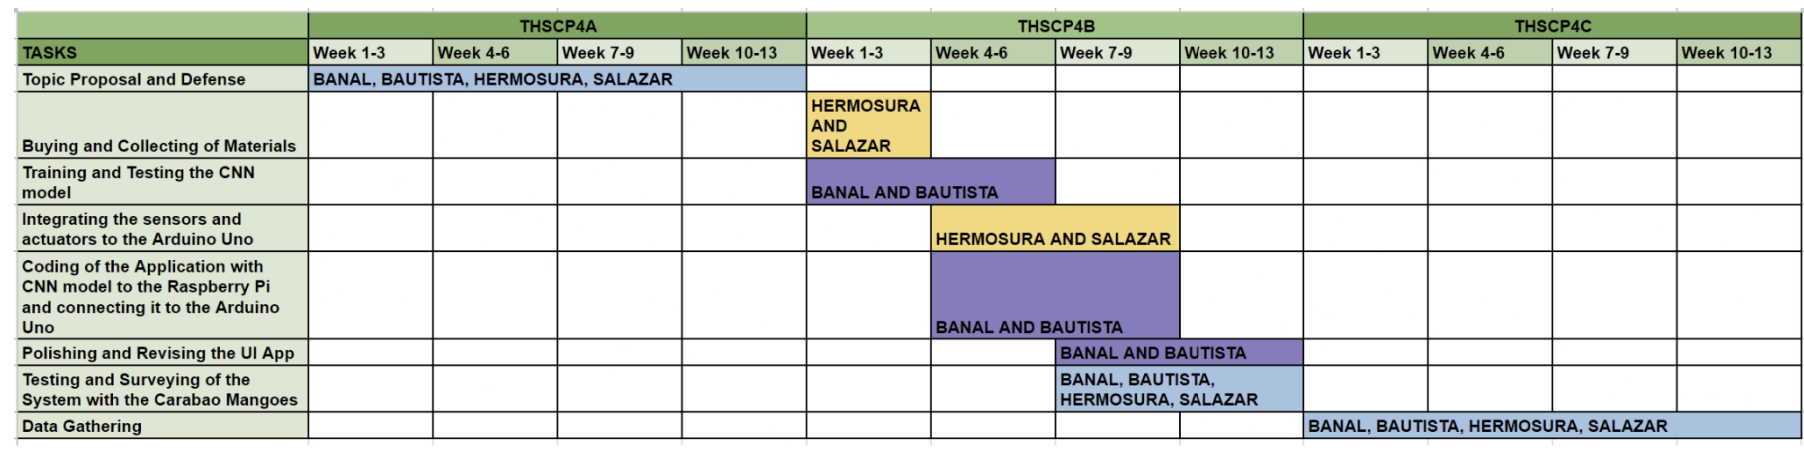
\includegraphics[width=1\textwidth]{ganttchart}
	\caption{Gantt Chart}
	\label{fig:img2}
\end{figure}

As seen above, Table~\ref{fig:img2} shows the Gantt Chart together with the assigned task. For the
first part of the THSCP4A, the group would primarily revise and fine tune Chapters 1
and 2 while also preparing for the defense. After that for THSCP4B, the yellow team
which consists of two members, Hermosura and Salazar, would start buying and
collecting the materials needed for assembling the prototype. While team yellow is
doing that, team purple which consists of Banal and Baustista would start training and
validating the \acr{cnn} model based on the Carabao mango image dataset. After that
integration of the sensors and actuators together with the integration of the \acr{cnn} model
and beginning of coding of the Application to the Raspberry Pi would be done. Once
that \acr{cnn} model is deployed and the Application works testing of the Carabao mangoes
to the prototype would be done. During THSCP4C, data gathering would be done
together with polishing and revising of the final paper.

\ifPhD
\section{Publication Plan}
\graytx{\blindtext}
\fi

\fi


\section{Overview of the \documentType}

There are seven succeeding chapters. To recall, chapter 1 involves the introduction of the
thesis topic containing the background of the study, previous studies, objectives and
deliverables, assumptions, scope, and delimitation, significance of the study, description
of the project together with the methodology, and Gantt chart and budget. Chapter 2
involves the existing articles, the lacking in their approaches, and the summary of
chapter 2. Chapter 3 involves the theoretical considerations of the thesis topic while
chapter 4 would consist of the design consideration involving the thesis topic. Chapter 5
would involve the research methodology containing the testing procedure and setup.
Chapter 6 would involve the results and discussion based on the methodology while
Chapter 7 would involve the conclusion, recommendations, and future suggestions.
